\documentclass[
  captions=tableheading,
]{scrartcl}

\usepackage{scrhack}

\usepackage[aux]{rerunfilecheck}

\usepackage{fontspec}

\usepackage[main=ngerman]{babel}

\usepackage{amsmath}
\usepackage{amssymb}
\usepackage{mathtools}

\usepackage[
  math-style=ISO,
  bold-style=ISO,
  sans-style=italic,
  nabla=upright,
  partial=upright,
]{unicode-math}

\usepackage[
  locale=DE,
  separate-uncertainty=true,
  per-mode=reciprocal,
  output-decimal-marker=.,
]{siunitx}

\usepackage{float}
\floatplacement{figure}{htbp}
\floatplacement{table}{htbp}

\usepackage[
  labelfont=bf,
  font=small,
  width=0.9\textwidth,
]{caption}

\usepackage{graphicx}
\usepackage{grffile}

\usepackage{booktabs}

\usepackage[
  unicode,
]{hyperref}
\usepackage{bookmark}


\begin{document}

\section{Messwerte und Auswertung}

Die Messdaten befinden sich in Tabelle~\ref{tab:data}.
Die Ergbenisse des Fits an die Funktion
\begin{equation}
  U(t) = a \sin(b t + c) + d
\end{equation}
sind
\begin{align}
  a &= \input{loesung-a.tex} \\
  b &= \input{loesung-b.tex} \\
  c &= \input{loesung-c.tex} \\
  d &= \input{loesung-d.tex} .
\end{align}
Die Messdaten und das Ergebnis des Fits sind in Abbildung~\ref{fig:plot} geplottet.

\begin{table}
  \centering
  \caption{Messdaten.}
  \label{tab:data}
  \begin{tabular}{
    S[table-format=3.0] 
    S[table-format=2.3]
    S[table-format=2.2]
    S[table-format=3.1]
    S[table-format=2.2]
    S[table-format=3.3]
    S[table-format=3.2]
    S[table-format=3.1]
    S[table-format=2.2]
  }
  \toprule
  & \multicolumn{4}{c}{Messung 1} & \multicolumn{4}{c}{Messung 2} \\
  \cmidrule(lr){2-5} \cmidrule(lr){6-9}
  {$\symup{\Delta} t \mathbin{/} \si{\second}$} &
  {$R_\text{Probe} \mathbin{/} \si{\ohm}$} &
  {$R_\text{Geh} \mathbin{/} \si{\ohm}$} &
  {$I \mathbin{/} \si{\milli\ampere}$} &
  {$U \mathbin{/} \si{\volt}$} &
  {$R_\text{Probe} \mathbin{/} \si{\ohm}$} &
  {$R_\text{Geh} \mathbin{/} \si{\ohm}$} &
  {$I \mathbin{/} \si{\milli\ampere}$} &
  {$U \mathbin{/} \si{\volt}$} \\
  \midrule
      0 & 22.220  & 22.34  &  80   &  8.5  &  22.220 &  22.34 &  80   &  8.5  \\
    60 & 22.457  & 22.63  &  80   &  8.5  &  23.445 &  23.92 &  81   &  8.5  \\
    60 & 22.707  & 22.98  &  80   &  8.5  &  24.838 &  24.75 &  81.6 &  8.54 \\
    60 & 22.960  & 23.31  &  81   &  8.5  &  25.944 &  26.23 &  81.6 &  8.54 \\
    60 & 23.190  & 23.61  &  81   &  8.5  &  27.039 &  27.01 &  81.9 &  8.57 \\
    60 & 23.445  & 23.92  &  81   &  8.5  &  32.014 &  30.87 & 186.6 & 19.59 \\
    120 & 23.926  & 24.19  &  81.6 &  8.54 &  35.079 &  36.63 & 141.3 & 14.84 \\
    120 & 24.294  & 24.32  &  81.6 &  8.54 &  38.024 &  40.20 & 142.0 & 14.93 \\
    120 & 24.838  & 24.75  &  81.6 &  8.54 &  40.780 &  43.15 & 142.4 & 15.00 \\
    300 & 25.944  & 26.23  &  81.6 &  8.54 &  43.497 &  46.97 & 142.5 & 15.02 \\
    300 & 27.039  & 27.01  &  81.9 &  8.57 &  46.106 &  47.65 & 142.4 & 15.00 \\
    300 & 32.014  & 30.87  & 186.6 & 19.59 &  48.597 &  49.09 & 142.4 & 15.00 \\
    300 & 35.079  & 36.63  & 141.3 & 14.84 &  50.993 &  51.27 & 142.4 & 15.02 \\
    300 & 38.024  & 40.20  & 142.0 & 14.93 &  53.370 &  53.74 & 142.5 & 15.03 \\
    300 & 40.780  & 43.15  & 142.4 & 15.00 &  55.710 &  56.09 & 142.5 & 15.03 \\
    300 & 43.497  & 46.97  & 142.5 & 15.02 &  57.989 &  58.31 & 142.5 & 15.03 \\
    300 & 46.106  & 47.65  & 142.4 & 15.00 &  60.228 &  60.48 & 142.7 & 15.07 \\
    300 & 48.597  & 49.09  & 142.4 & 15.00 &  62.476 &  62.64 & 142.9 & 15.08 \\
    300 & 50.993  & 51.27  & 142.4 & 15.02 &  64.677 &  65.04 & 143.0 & 15.09 \\
    300 & 53.370  & 53.74  & 142.5 & 15.03 &  66.858 &  67.24 & 143.0 & 15.10 \\
    300 & 55.710  & 56.09  & 142.5 & 15.03 &  69.000 &  69.41 & 143.0 & 15.10 \\
    300 & 57.989  & 58.31  & 142.5 & 15.03 &  71.158 &  71.57 & 143.0 & 15.10 \\
    300 & 60.228  & 60.48  & 142.7 & 15.07 &  73.263 &  73.73 & 143.0 & 15.10 \\
    300 & 62.476  & 62.64  & 142.9 & 15.08 &  75.371 &  75.86 & 143.0 & 15.10 \\
    300 & 64.677  & 65.04  & 143.0 & 15.09 &  77.485 &  77.94 & 143.1 & 15.12 \\
    300 & 66.858  & 67.24  & 143.0 & 15.10 &  79.518 &  79.76 & 143.1 & 15.12 \\
    300 & 69.000  & 69.41  & 143.0 & 15.10 &  81.545 &  81.44 & 143.0 & 15.13 \\
    300 & 71.158  & 71.57  & 143.0 & 15.10 &  83.514 &  83.01 & 143.0 & 15.13 \\
    300 & 73.263  & 73.73  & 143.0 & 15.10 &  85.352 &  84.58 & 143.0 & 15.13 \\
    300 & 75.371  & 75.86  & 143.0 & 15.10 &  87.211 &  87.33 & 143.0 & 15.13 \\
    300 & 77.485  & 77.94  & 143.1 & 15.12 &  89.163 &  89.62 & 143.2 & 15.12 \\
    300 & 79.518  & 79.76  & 143.1 & 15.12 &  91.131 &  91.25 & 143.2 & 15.12 \\
    300 & 81.545  & 81.44  & 143.0 & 15.13 &  93.034 &  92.80 & 143.2 & 15.12 \\
    300 & 83.514  & 83.01  & 143.0 & 15.13 &  94.883 &  94.32 & 143.2 & 15.12 \\
    300 & 85.352  & 84.58  & 143.0 & 15.13 &  96.705 &  97.07 & 143.2 & 15.12 \\
    300 & 87.211  & 87.33  & 143.0 & 15.13 &  98.624 &  98.98 & 143.2 & 15.12 \\
    300 & 89.163  & 89.62  & 143.2 & 15.12 & 100.507 & 100.60 & 143.2 & 15.12 \\
    300 & 91.131  & 91.25  & 143.2 & 15.12 & 102.369 & 102.58 & 143.2 & 15.12 \\
    300 & 93.034  & 92.80  & 143.2 & 15.12 & 104.261 & 104.55 & 143.2 & 15.12 \\
    300 & 94.883  & 94.32  & 143.2 & 15.12 & 106.138 & 106.44 & 143.2 & 15.12 \\
  \bottomrule
\end{tabular}

\end{table}

\begin{figure}
  \centering
  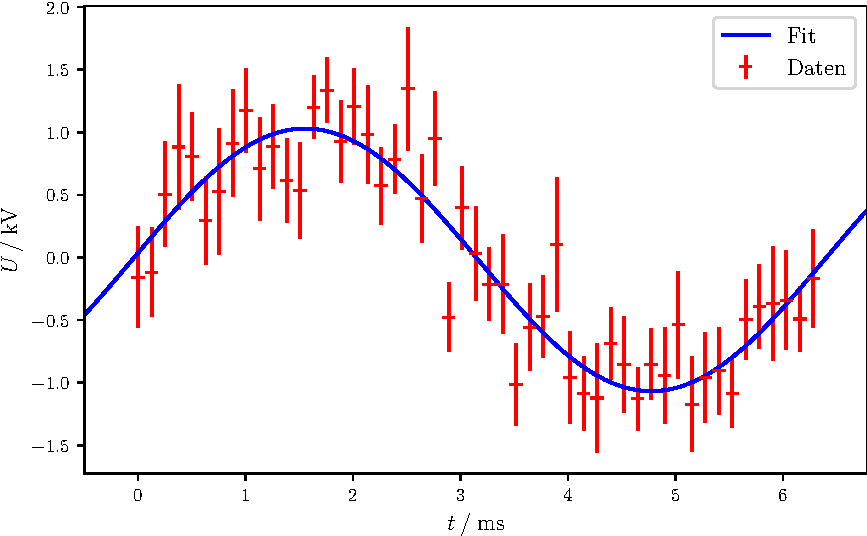
\includegraphics{loesung-plot.pdf}
  \caption{Messdaten und Fitergebnis.}
  \label{fig:plot}
\end{figure}

\end{document}
